% See the REVTeX 4 README file
% It also requires running BibTeX. The commands are as follows:
%
%  1)  latex Report.tex
%  2)  bibtex Report
%  3)  latex Report.tex
%  4)  latex Report.tex
%
\documentclass[%
 reprint,
%superscriptaddress,
%groupedaddress,
%unsortedaddress,
%runinaddress,
%frontmatterverbose, 
%preprint,
%preprintnumbers,
%nofootinbib,
%nobibnotes,
%bibnotes,
 amsmath,amssymb,
 aps,
%pra,
%prb,
%rmp,
%prstab,
%prstper,
%floatfix,
]{revtex4-2}

\usepackage{graphicx}% Include figure files
\usepackage{physics, amsmath, gensymb, multirow}
\usepackage{dcolumn}% Align table columns on decimal point
\usepackage{bm}% bold math
%\usepackage{hyperref}% add hypertext capabilities
%\usepackage[mathlines]{lineno}% Enable numbering of text and display math
%\linenumbers\relax % Commence numbering lines
\usepackage{url}

%\usepackage[showframe,%Uncomment any one of the following lines to test 
%%scale=0.7, marginratio={1:1, 2:3}, ignoreall,% default settings
%%text={7in,10in},centering,
%%margin=1.5in,
%%total={6.5in,8.75in}, top=1.2in, left=0.9in, includefoot,
%%height=10in,a5paper,hmargin={3cm,0.8in},
%]{geometry}

\begin{document}

\preprint{APS/123-QED}

\title{Comparative Analysis of Quantum Algorithm for \\Portfolio Optimization: A Study of VQE}% Force line breaks with \\
%\thanks{A footnote to the article title}%

\author{Michael Cai, Justin Beltran, Chaipat Tirapongprasert, Hyeon-Tae Hwang, Yoonsuk Choi, Farhaan Siddiqui}

\affiliation{Columbia University}

\date{\today}
\begin{abstract}
This supplementary file complements the slideshow for the NYC Quantum Hackathon and is in no way emanating the knowledge presented in those of a paper. We began by using key papers to define and setup the initial problem and implement our own programs to verify and test against reigning classical models. This supplemental resource explores the strengths and weaknesses of the Variational Quantum Eigensolver (VQE), with a focus on its applicability to real-world financial scenarios \cite{Cerezo2021}. Additionally, it discusses the computational complexity, convergence rates, and potential advantages these quantum algorithms offer over classical methods in optimizing asset allocation and risk management. Case studies are presented to demonstrate the performance of each algorithm on benchmark portfolio optimization problems, highlighting their scalability and efficiency in handling large datasets. The analysis aims to identify the specific conditions under which each algorithm excels, offering insights into their practical implementation within financial institutions.
\end{abstract}

%\keywords{Suggested keywords}%Use showkeys class option if keyword
                              %display desired
\maketitle

%\tableofcontents

\section{\label{sec:level1}Introduction%\protect\\ The line break was forced \lowercase{via} \textbackslash\textbackslash
}
Portfolio optimization, rooted in the principles of Modern Portfolio Theory (MPT) as introduced by Harry Markowitz in 1952 \cite{Markowitz1952}, seeks to maximize expected returns while minimizing risk through the strategic allocation of assets. This process typically involves the use of a covariance matrix to analyze the relationships between various assets, alongside metrics such as the Sharpe ratio to evaluate performance \cite{Sharpe1964}. However, the complexity of these optimization problems often categorizes them as NP-hard, presenting significant challenges in computational feasibility \cite{Boyd2004}. Traditional methods, including Monte Carlo simulations and maximum diversification techniques, struggle to efficiently navigate the vast solution space inherent in large portfolios.

In recent years, advancements in quantum computing have opened new avenues for tackling these complex optimization problems \cite{Moll2018}. Notable contributions from organizations such as IBM and D-Wave have demonstrated the potential of quantum algorithms to outperform classical approaches \cite{Hodson2019}. Quantum algorithms, such as the Variational Quantum Eigensolver (VQE) \cite{Peruzzo2014, McClean2016}, offer unique advantages in optimizing asset allocation and risk management by leveraging quantum superposition and entanglement.

These techniques can leverage entanglement to perform calculations, significantly reducing the time required to identify optimal strategies in dynamic market conditions \cite{Cerezo2021}. As the financial industry continues to embrace these innovations, we can expect a paradigm shift in how investment strategies are developed and executed, ultimately leading to more robust and resilient portfolios. Thus, it makes sense that the motivation behind this challenge lies in understanding the potential of quantum computing to revolutionize traditional financial models and enhance decision-making processes through an analysis of time and space complexity as well as scalability.
\section{Theory}
\subsection{Variational Quantum Algorithm Overview}

To intuitively understand the algorithm, the Variational Quantum Eigensolver is defined based on the 2022 paper written by Jules Tilly \cite{Tilly2022}. We will then introduce the IBM Qiskit implementation through it.

The goal of VQE is to optimize an upper bound for the lowest possible expectation value of an observable with respect to a trial wavefunction. Specifically, by presenting a Hamiltonian $\hat{H}$ and a trial wavefunction $\ket{\psi}$, the ground state energy associated with this Hamiltonian, denoted as $E_0$, is constrained by the inequality 
\[
E_0 \leq \frac{\bra{\psi}\hat{H}\ket{\psi}}{\bra{\psi}\psi\rangle}. 
\tag{1}
\]
Consequently, the primary aim of the Variational Quantum Eigensolver (VQE) is to ascertain a parameterization of $\ket{\psi}$ that minimizes the expectation value of the Hamiltonian. This expectation value serves as an upper limit for the ground state energy and, in an ideal scenario, should be indistinguishable from the true ground state energy to the desired precision level. From a mathematical perspective, our objective is to derive an approximation of the eigenvector $\ket{\psi}$ of the Hermitian operator $\hat{H}$ that corresponds to the lowest eigenvalue, $E_0$. 

To reformulate this minimization endeavor into a task amenable to execution on a quantum computer, it is imperative to begin by defining an ansatz wavefunction that can be formed into a executable circuit on a quantum device through a succession of quantum gates. Since only unitary operations or measurements can be conducted on a quantum computer, this is accomplished by employing parameterized unitary operations. 

Thus, we articulate $\ket{\psi}$ as the result of applying a generic parameterized unitary $U(\theta)$ to an initial state representing $N$ qubits, with $\theta$ representing a set of parameters that assume values within the interval $(-\pi, \pi]$. The qubit register is typically initialized as $\ket{0}^{\otimes N}$ for simplicity, although low-depth operations may be executed for alternative initial states prior to the application of the unitary. Note, we will denote $\ket{0}^{\otimes N}$ as $\ket{0}$ for simplification of the equations. Acknowledging that $\ket{\psi}$ (and similarly any $U(\theta)\ket{\psi}$) must inherently be a normalized wavefunction, we can reformulate the VQE optimization challenge as 
\[
E_{\text{VQE}} = \min_{\theta} \bra{0}U^\dagger(\theta) \hat{H} U(\theta)\ket{0}.
\tag{2}
\]
Equation (2) is commonly referred to as the cost function of the VQE optimization framework, a term derived from the realms of machine learning and optimization literature. 

We can extend this exposition by expressing the Hamiltonian in a form that is directly measurable on a quantum computer, represented as a weighted sum of spin operators. Observables that are conducive to direct measurement on a quantum device are tensor products of spin operators (Pauli operators). We may define these as Pauli strings: 
\[
\hat{P}_a \in \{I, X, Y, Z\}^{\otimes N},
\]
where $N$ signifies the number of qubits utilized to model the wavefunction. The Hamiltonian can be reformulated as 
\[
\hat{H} = \sum_a w_a \hat{P}_a,
\tag{3}
\]
where $w_a$ denotes a set of weights, and $P$ represents the total number of Pauli strings within the Hamiltonian. Consequently, Equation (2) transforms into 
\[
E_{\text{VQE}} = \min_{\theta} \sum_a w_a \bra{0}U^\dagger(\theta) \hat{P}_a U(\theta)\ket{0},
\tag{4}
\]
wherein the hybrid nature of the VQE becomes distinctly evident: each term 
\[
E_{P_a} = \bra{0}U^\dagger(\theta) \hat{P}_a U(\theta)\ket{0}
\]
corresponds to the expectation value of a Pauli string $\hat{P}_a$ and can be computed on a quantum device, while the summation and minimization 
\[
E_{\text{VQE}} = \min_{\theta} \sum_a w_a E_{P_a}
\]
are executed on a classical computer.

\begin{figure*}
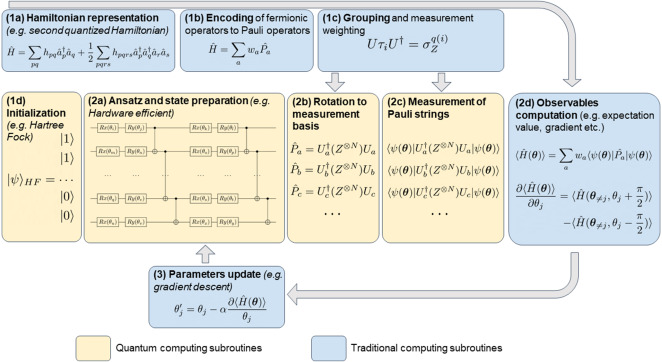
\includegraphics[width=16cm]{Pictures/VQE Algorithm.jpg}
\caption{\label{fig:pipeline} The VQE Pipeline — Illustrative formulas do not guarantee best practices. (1) Pre-processing: (a) Hamiltonian representation: Initial step defining basis functions for Hamiltonian as a quantum observable; (b) Encoding: Second step encoding Hamiltonian into measurable operators on a Quantum Computer via qubit wavefunction, mapping fermionic to spin operators; (c) Grouping and measurement strategy: Third step involves grouping operators for simultaneous measurement, necessitating circuit additions for basis rotation and establishing measurement weighting; (d) State initialization: Final pre-processing step determining the state initialization for the ansatz — (2) The VQE loop: (a) Ansatz and trial state preparation: Initial step applying ansatz to initialized qubit register, requiring parameter initialization before the first iteration; (b) Basis rotation and measurement: Prepared trial wave function is rotated into the measurement basis or a diagonal basis of specific Pauli strings; (c) Observable computation: Expectation value computation is determined by the optimization strategy, involving weighted summation on conventional hardware or machine learning techniques; (d) Parameters update: Updates to ansatz parameters are computed based on observables and optimization strategies, initiating a new VQE iteration — (3) Post-processing, Error mitigation: Additional computation layer aims to reduce quantum noise impact on measurement results \cite{Tilly2022}.}
\end{figure*}

\textbf{Hamiltonian construction and representation:} As shown in Figure \ref{fig:pipeline}, the first step in the VQE is defining the system for which we want to find the ground state. In the context of portfolio optimization, this could be a Hamiltonian representing an optimization problem based on Markowitz's mean-variance model, where the objective is to minimize the portfolio risk (variance) while maximizing the return. The Hamiltonian is constructed by mapping the cost function, including the covariance matrix for asset returns and expected returns, into a quantum observable. The choice of representation, such as encoding the asset selection in binary or using fractional shares, significantly impacts both the accuracy and the computational cost of the solution. Additionally, constraints such as budget limits or asset allocation restrictions must be incorporated into the Hamiltonian to ensure feasible portfolio solutions.

\textbf{Encoding of operators:} Since qubit registers can only measure observables in the Pauli basis, the problem's cost function, expressed as a classical function of asset returns, must be encoded into Pauli operators. This process involves translating the classical optimization problem into a quantum optimization problem, affecting the efficiency of the computation. Different encodings, such as binary or unary encoding of asset weights, influence the number of qubits required and the number of Pauli terms generated, impacting the circuit depth and performance.

\textbf{Measurement strategy and grouping:} To efficiently extract the required expectation values of the cost function (e.g., portfolio variance and return), measurements must be organized to minimize the number of repetitions (shots). Techniques such as grouping commuting Pauli strings allow multiple terms in the Hamiltonian to be measured simultaneously, optimizing the measurement process. Further optimization can be achieved by leveraging the structure of the covariance matrix and expected returns, potentially reducing the number of measurements required.

\textbf{Ansatz and state preparation:} The ansatz, a parameterized quantum circuit, is used to generate the trial portfolio allocation. Its expressibility determines how well it can approximate the optimal portfolio, while its trainability impacts how efficiently it can be optimized. A good ansatz balances expressibility and trainability while keeping circuit depth manageable, which is important for noise resilience on near-term devices.

\textbf{Parameter optimization:} The ansatz parameters, representing asset weights or allocation proportions, are iteratively updated to minimize the portfolio risk subject to constraints, such as achieving a target return. The optimization method affects the number of measurements, convergence speed, and resilience to issues like barren plateaus. Specialized optimizers can be designed to handle the specific challenges of portfolio optimization problems, such as gradient-free methods or those tailored to handle large portfolios.

\textbf{Error mitigation:} Given the presence of quantum noise on current devices, error mitigation is crucial for VQE applications in portfolio optimization. These techniques reduce the impact of noise through post-processing of measurement data, allowing for more accurate portfolio allocations without relying on full quantum error correction.

\subsection{Quantum Formulation of Portfolio Optimization}
According to Hodson et al. \cite{Hodson2019}, ``the portfolio optimization (PO) problem lies within the class of quadratic optimization problems. To make it quantum-native, it must be converted into a Quadratic Unconstrained Binary Optimization (QUBO) problem, where the target vector is expressed as a vector of zeros and ones, avoiding constraints.

The binary conversion matrix $C$ is constructed with binarizing elements $d_i$ for each asset $i$ depending on the price $P_i$. Hence:

\[
n_{\text{max}}^i = \text{Int}\left(\frac{B}{P_i}\right),
\]

where the operation Int stands for the integer part, and

\[
d_i = \text{Int}\left(\log_2 n_{\text{max}}^i\right),
\]

such that

\[
n_i = \sum_{j=0}^{d_i} 2^j b_{i,j}.
\]

The overall dimension of the binarized target vector $b = \left[b_{1,0}, \dots, b_{1,d_1}, \dots, b_{N,0}, \dots, b_{N,d_N}\right]$ is given by:

\[
\text{dim}(b) = \sum_{i=1}^{N} (d_i + 1).
\]

Conveniently, the encoding matrix $C$ is defined as follows:

\[
C = \begin{pmatrix}
2^0 & \cdots & 2^{d_1} & 0 & \cdots & 0 & \cdots & 0 \\
0 & \cdots & 0 & 2^0 & \cdots & 2^{d_2} & \cdots & 0 \\
\vdots & & \vdots & & \vdots & & \vdots & \vdots \\
0 & \cdots & 0 & \cdots & 0 & 2^0 & \cdots & 2^{d_N}
\end{pmatrix}.
\]

Thus, the conversion can be written in short notation as $n = Cb$. The problem can be redefined in terms of the binary vector $b$, applying the encoding matrix:

\[
\mu'' = C^T \mu', \quad \Sigma'' = C^T \Sigma' C, \quad P'' = C^T P'.
\]

The problem falls into binary quadratic optimization with the constraint given by the total budget. It cannot be directly cast into quantum operators, so the constraint must be converted into a penalty term in the objective function. Hence, the QUBO problem is:

\[
\max_b L(b) : \max_b \left( \mu''^T b - b^T \Sigma'' b - \lambda \left(P''^T b - 1 \right)^2 \right),
\tag{13}
\]

where $\lambda$ is the penalty coefficient, and the problem now falls into the class of binary quadratic optimization problems.

There is a strong connection, technically an isomorphism, between QUBO problems and the Ising Hamiltonian. The Ising Hamiltonian was originally constructed to understand the microscopic behavior of magnetic materials, particularly phase transitions. However, its relative simplicity and natural mapping to QUBO problems have made the Ising model a fundamental benchmark beyond quantum physics. To convert Eq. (13) into an Ising model, we expand it into its components as follows:

\[
L(b) = \sum_i \mu''_i b_i - \sum_{i,j} \Sigma''_{i,j} b_i b_j - \lambda \left(\sum_i P''_i b_i - 1\right)^2.
\tag{14}
\]

In the Ising model, spin variables $s_i \in \{-1, 1\}$ replace the binary variables $b_i \in \{0, 1\}$. The transformation $b_i \rightarrow \frac{1 + s_i}{2}$ is applied, and the coefficients are re-arranged to obtain the Ising objective function:

\[
L(s) = \sum_i h_i s_i + \sum_{i,j} J_{i,j} s_i s_j + \lambda \left( \sum_i \pi_i s_i - \beta \right)^2,
\tag{15}
\]

subject to $s_i \in \{-1, 1\} \ \forall \ i$.

The Ising objective function above can now be transformed into a quantum Hamiltonian. The eigenvalues of Pauli operators $Z$ are $\pm 1$, making them suitable for describing classical spin variables $s_i$. Additionally, the two-body interaction term between spins can be modeled using tensor products of Pauli operators, specifically $Z_i \otimes Z_j$. The resulting quantum Ising Hamiltonian reads:

\[
H = \sum_i h_i Z_i + \sum_{i,j} J_{i,j} Z_i \otimes Z_j + \lambda \left( \sum_i \pi_i Z_i - \beta \right)^2.
\tag{16}
\]

In this formulation, $h_i$, $J_{i,j}$, and $\pi_i$ are the components of the transformed objective function. The Hamiltonian $H$ describes the system’s energy, and the task is to find the ground state, i.e., the eigenstate of $H$ that corresponds to the minimum energy eigenvalue."



\section{Methodology}
\subsection{Portfolio Choices}
\begin{figure}[b]
\includegraphics[width=1\columnwidth]{Pictures/Random Data Provider.png}
\caption{\label{fig:data} 
This figure shows the price evolution of 25 randomly generated stocks over a specified time horizon (measured in days). Each line corresponds to a distinct stock (STOCK0 to STOCK24).
}
\end{figure}
The selection of the portfolio is considered based on the inherent runtime complexity that VQE has. The magnitude of the portfolio holds significance for Qiskit implementation, given the inherent complexity of $2^N$. Accordingly, we will opt for 20 out of 25 stocks, as IBM computing systems and simulators possess the capability to execute such computations with relative ease. For the present experiment, we shall utilize data sets supplied within the IBM Qiskit Portfolio Optimization version \texttt{0.6.1}. A \texttt{RandomDataProvider} will be employed to pseudo-randomly produce simulated stock market data as shown in Figure 2. 

In order to implement the QUBO presented, each portfolio is endowed with designated data utilized to generate anticipated returns and the covariance matrix derived from (stochastic) time-series data, specifically for \texttt{RandomDataProvider(start=datetime.datetime(2023, 1, 1), end=datetime.datetime(2023, 1, 30))}. The covariance matrix provides insights into how the returns of different assets move together. To calculate the covariance between two assets \( A \) and \( B \):

\[
\text{Cov}(A,B) = \frac{1}{n-1} \sum_{t=1}^{n} \left( R_{A,t} - \bar{R}_A \right)\left( R_{B,t} - \bar{R}_B \right)
\]

where \( R_A \) and \( R_B \) are the returns of assets \( A \) and \( B \), and \( \bar{R}_A \) and \( \bar{R}_B \) are the mean returns of assets \( A \) and \( B \). In a portfolio of multiple assets, the covariance matrix \( \Sigma \) is constructed by computing the pairwise covariances between all assets.

For every stock or asset encompassed within your portfolio, one acquires: Adjusted closing prices (which incorporate dividends and stock splits) and the temporal scope within which one intends to scrutinize the returns (e.g., daily, monthly, or annually). The Variational Quantum Eigensolver (VQE) algorithm will determine whether to select a particular stock or not, indicating its lack of knowledge regarding the percentage allocation. This aspect necessitates consideration in a separate context, and is not elaborated upon herein.


\subsection{Qiskit Implementation}

\begin{figure}[b]
\includegraphics[width=1\columnwidth]{Pictures/Gradient Analysis.png}
\caption{\label{fig:data} This figure compares Finite Difference, SPSA, Natural Gradient, and Analytic Gradient with step size \( \mu = 0.1 \). The estimated energy decreases quickly within the first 10 iterations for all methods.
}
\includegraphics[width=1\columnwidth]{Pictures/SU2_conv.png}
\caption{\label{fig:data} Convergence Analysis of the SU2 Circuit using three entanglement protocols: linear, cyclic, and full.
}
\end{figure}

\begin{figure}[b]

\includegraphics[width=1\columnwidth]{Pictures/ZZ_conv.png}
\caption{\label{fig:data} Convergence Analysis of the ZZ Feature Map Circuit using three entanglement protocols: linear, cyclic, and full.
}
\includegraphics[width=1\columnwidth]{Pictures/TwoL_conv.png}
\caption{\label{fig:data} Convergence Analysis of the Two Local Circuit using three entanglement protocols: linear, cyclic, and full.
}
\end{figure}


The utilization of the \texttt{QuadraticProgram} from the \texttt{qiskit\_optimization.problems} library, specifically version 0.6.1, is noted. The process of converting an optimization problem into a Hamiltonian mirrors the implementation provided by IBM's Qiskit framework.

We shall elucidate the code utilized for the purpose of translation. First, we invoke the function \texttt{PortfolioOptimization}, which encapsulates the anticipated returns, covariance matrix, and associated risk factors. This data is subsequently formatted into an unconstrained structure employing the converter method tailored for our quadratic program. Then, we proceed to translate our quadratic unconstrained binary optimization (QUBO) problem into the Ising model through the application of \texttt{qubo.to\_ising()}, a process facilitated by Qiskit's portfolio optimization methodology.

There exists a plethora of gradient descent methodologies available for selection, encompassing finite-difference gradient, Quantum Natural Gradient, Analytic Gradient (Parametric Shift Rule), and Simultaneous Perturbation Stochastic Approximation (SPSA). Our investigation employs the parametric shift rule, which represents the analytic gradient approach.

Assume each parameter $\theta_i$ contributes to the ansatz through a gate of the form:
\[
U_i(\theta) = \exp\left(-j \frac{\theta_i}{2} P_i\right)
\]
where $P_i$ is a Pauli string. The gradient of the expectation value $V(\theta)$ with respect to $\theta_i$ is:
\[
\frac{\partial V(\theta)}{\partial \theta_i} = \frac{V\left(\theta + \frac{\pi}{2} e_i\right) - V\left(\theta - \frac{\pi}{2} e_i\right)}{2}
\]
This can be derived as follows:

Let $\theta = \{\theta_1, \dots, \theta_M\}$ for each $k = 1, \dots, M$:
\[
U(\theta) = V(\theta_{-k}) U_k(\theta_k) W(\theta_{-k})
\]
where $\theta_{-k}$ denotes all parameters except $\theta_k$. The expectation value of the observable $O$ with respect to the state $\Psi(\theta)$ is given by:
\[
\langle O \rangle | \Psi(\theta) \rangle = \langle \Psi(\theta) | O | \Psi(\theta) \rangle = \langle 0 | U(\theta)^* O U(\theta) | 0 \rangle
\]
Continuing this analysis, the derivative of $\langle O \rangle | \Psi(\theta) \rangle$ with respect to $\theta_k$ can be written as:
\begin{align}
\frac{\partial \langle O \rangle | \Psi(\theta) \rangle}{\partial \theta_k} &= \langle \phi_k | \frac{\partial U_k(\theta_k)^*}{\partial \theta_k} R_k U_k(\theta_k) | \phi_k \rangle \nonumber \\
&\quad + \langle \phi_k | U_k(\theta_k)^* R_k \frac{\partial U_k(\theta_k)}{\partial \theta_k} | \phi_k \rangle
\end{align}

where $U_k(\theta_k)$ is expressed as:
\[
\frac{\partial U_k(\theta_k)}{\partial \theta_k} = \frac{\partial}{\partial \theta_k} \exp\left(-j \frac{\theta_k}{2} P_k\right) = -j \frac{1}{2} \exp\left(-j \frac{\theta_k}{2} P_k\right)
\]
Thus, the derivative becomes:
\[
\frac{\partial U_k(\theta_k)}{\partial \theta_k} = -j \frac{1}{2} P_k U_k(\theta_k)
\]
Finally, the derivative of the unitary $U_k(\theta_k)$ is given by:
\[
\frac{\partial U_k(\theta_k)}{\partial \theta_k} = (I - j P_k) U_k(\theta_k) = S^+_k
\]

This gradient is employed based on its implementation within a Variational Quantum Eigensolver (VQE) circuit, recognized as the most expedient gradient methodology. We conducted experiments utilizing arbitrary Hamiltonians, and the results in Figure 4 indicated that the Efficient SU(2) Linear emerged as the most efficient.

The Variational Quantum Eigensolver (VQE) in our implementation is run using the \texttt{qiskit} framework, specifically leveraging a quantum simulator backend. The following steps outline the VQE setup:

1. \textbf{Quantum Backend:} The quantum computations are performed using a quantum simulator, indicated by the import of \texttt{Sampler} from the \texttt{qiskit\_aer} library.

2. \textbf{Ansatz Circuits:} The parameterized quantum circuits (PQC) used in the VQE are chosen from three common quantum circuits: \texttt{EfficientSU2}, \texttt{ZZFeatureMap}, and \texttt{TwoLocal}, each supporting various entanglement structures (linear, circular, and full). These circuits form the basis of the ansatz, which is iteratively optimized during the VQE process.

3. \textbf{Optimization Method:} Classical optimization techniques are employed to minimize the expectation value of the Hamiltonian. The VQE implementation incorporates optimizers such as \texttt{COBYLA}, \texttt{GradientDescent}, and \texttt{ParamShiftEstimatorGradient}. These optimizers iteratively adjust the parameters of the ansatz circuits to converge on the minimum eigenvalue of the Hamiltonian. 

\subsection{IBM Hardware Implementation}

\begin{figure}[b]
\includegraphics[width=1\columnwidth]{Pictures/Transpiler Steps.png}
\caption{\label{fig:data} Transpilation is the process of rewriting a given input circuit to match the topology of a specific quantum device, and/or to optimize the circuit for execution on present day noisy quantum systems.}
\end{figure}
\begin{figure}[b]
\includegraphics[width=1\columnwidth]{Pictures/singlequbiterror.png}
\caption{\label{fig:data} This figure presents the singular qubit gate linear decay of the error rate as a function of the number of gates, \(k\), with varying numbers of qubits \(r\).
}
\includegraphics[width=1\columnwidth]{Pictures/twoqubiterror.png}
\caption{\label{fig:data}  This figure presents the exponential decay of \(k\)-GHZ states as a function of the number of gates, \(k\), with varying numbers of qubits per gate \(r\).
}
\end{figure}

Transpilation within the domain of quantum computing denotes the procedure of converting a quantum circuit into a corresponding circuit that aligns with the limitations imposed by the target computational hardware \cite{Moll2018}. Specifically, in the context of IBM Quantum computing systems, the hardware consists of superconducting qubits characterized by distinct connectivity patterns and varying error rates associated with quantum gates shown in Figure 7. Transpilation entails the mapping of logical qubits to their corresponding physical qubits, thereby ensuring that the quantum operations are executable within the constraints of the hardware topology. Gate decomposition involves substituting unsupported gates (such as multi-qubit gates) with operations that are compatible, utilizing native gates. Optimization refers to the process of minimizing both the circuit depth (the number of sequential operations) and the total gate count, all while taking into account qubit connectivity and the error rates associated with the gates.

Quantum computing systems developed by IBM exhibit limitations in qubit connectivity, wherein not all qubits are capable of direct interaction. The process of transpilation takes this limitation into account and seeks to optimize the arrangement of qubits in order to minimize superfluous swaps. The error rates associated with different gates are not uniform. As shown in Figure 8 and 9, single-qubit gates typically demonstrate lower error rates and can be executed with greater reliability compared to two-qubit gates, which display an exponential increase in error rates. Consequently, the transpiler may strive to curtail the utilization of two-qubit gates.

We will use transpilation and the methodologies for its optimization via ibm\_brisbane, accompanied by a demonstrative test. We shall conduct a portfolio optimization involving four distinct assets on ibm\_brisbane alongside various other quantum computing platforms to evaluate the comparative performance of these quantum systems. Subsequently, we will ascertain the specific factors contributing to the superior performance of certain quantum computers over others. For instance, a comparative analysis of ibm\_brisbane with ibm\_kyoto and additional systems will be undertaken. This investigation will provide insights into the scenarios where quantum portfolio optimization exhibits scalability and advantages regarding time and space complexity in relation to superconducting circuits.

\section{Performance Metrics and Evaluation}
The performance of the VQE is going to be compared to baselines in order to check its performance. Additionally, we will be testing with respect to industry standard baselines for portfolio optimization. It will make sense for us to use basic ones that will do simple functions since more complex analysis will not be fruitful as a comparison to VQE. Additionally, due to the limitations of the binary operation of VQE of picking 0 or 1, the comparison will be skewed due to the fact that all classical situations can buy percentages of the whole.

\subsection{Global Minimum Variance Portfolio (GMVP)}

Global Minimum Variance Portfolio performs by finding the minimum variance in the set of all possible portfolio combinations. In other terms,
minimize the portfolio variance:
\[
\text{Minimize} \quad V(w) = w^\top \Sigma w
\]
Where:
\begin{itemize}
    \item \( w = (w_1, w_2, \dots, w_n) \) is the vector of asset weights,
    \item \( \Sigma \) is the covariance matrix of asset returns,
    \item \( V(w) \) represents the portfolio variance, which is a quadratic form of the weights and the covariance matrix.
\end{itemize}

The optimization is subject to the following constraints:

1. \textbf{Budget constraint:} The sum of the asset weights must equal 1:
\[
\sum_{i=1}^{n} w_i = 1
\]
This ensures that the full portfolio is allocated (100\%).

2. \textbf{Bounds on weights:} The weights are constrained between 0 and 1, not allowing for short selling:
\[
0 \leq w_i \leq 1 \quad \text{for all} \quad i = 1, 2, \dots, n
\]
This allows for long positions (positive weights) only. The expected return of the optimal portfolio is calculated as:
\[
\text{Expected Return} = w^\top \mu
\]
Where \( \mu = (\mu_1, \mu_2, \dots, \mu_n) \) is the vector of expected returns for each asset.

We are running this as a baseline since in industry, this is the least riskiest portfolio possible given the constraints of buying 20 of 25 stocks. Thus, any performance of any other algorithm should give a greater expected return \cite{Boyd2004}.

\subsection{Minimum Eigensolver}

Additionally, we will employ the Minimum Eigensolver to minimize variance, utilizing the same minimization and variance framework. The optimization process leverages the optimization module from qiskit to select the optimal portfolio of assets, aiming to maximize returns while minimizing the risk of the portfolio. Specifically, the NumPyMinimumEigensolver and MinimumEigenOptimizer are used to determine the minimum eigenvalue of the problem, which represents the optimal solution.


\subsection{Monte Carlo Simulation}
The Monte Carlo Simulation calculates all possible portfolio combinations and picks the best one given the constraints.

Let:
\begin{itemize}
    \item \( n = 25 \) represent the number of assets (qubits),
    \item \( \mathbf{w} = (w_1, w_2, \dots, w_n) \) represent the weights of the portfolio, where \( w_i \) is the allocation to asset \( i \),
    \item \( \mathbf{r} = (r_1, r_2, \dots, r_n) \) represent the vector of expected returns for each asset,
    \item \( \Sigma \) represent the covariance matrix of asset returns,
    \item \( \lambda \) represent the risk factor, which penalizes high-risk portfolios,
    \item \( B \) represent the total budget for the portfolio.
\end{itemize}

For each iteration \( k = 1, 2, \dots, N \), generate random portfolio weights \( \mathbf{w}^{(k)} \) such that:
\[
w_i^{(k)} \in [0, 1] \quad \text{and} \quad \sum_{i=1}^{n} w_i^{(k)} = 1
\]
The weights are then scaled by the budget \( B \):
\[
\mathbf{w}^{(k)} = B \cdot \mathbf{w}^{(k)}
\]
The expected return of the portfolio in iteration \( k \) is:
\[
R^{(k)} = \mathbf{w}^{(k)^\top} \mathbf{r} = \sum_{i=1}^{n} w_i^{(k)} r_i
\]
The risk (variance) of the portfolio in iteration \( k \) is calculated as:
\[
\text{Risk}^{(k)} = \mathbf{w}^{(k)^\top} \Sigma \mathbf{w}^{(k)}
\]
The standard deviation (volatility) is:
\[
\text{StdDev}^{(k)} = \sqrt{\text{Risk}^{(k)}}
\]
The adjusted return is computed by penalizing the portfolio's risk using the risk factor \( \lambda \):
\[
\text{AdjustedReturn}^{(k)} = R^{(k)} - \lambda \cdot \text{Risk}^{(k)}
\]
The best portfolio is the one that maximizes the adjusted return:
\[
\mathbf{w}^* = \arg \max_{\mathbf{w}^{(k)}} \left( R^{(k)} - \lambda \cdot \text{Risk}^{(k)} \right)
\]
The expected return of the best portfolio is:
\[
R^* = \mathbf{w}^{*^\top} \mathbf{r}
\]
The risk of the best portfolio is:
\[
\text{Risk}^* = \mathbf{w}^{*^\top} \Sigma \mathbf{w}^*
\]

\section{Results}

\begin{figure}[b]
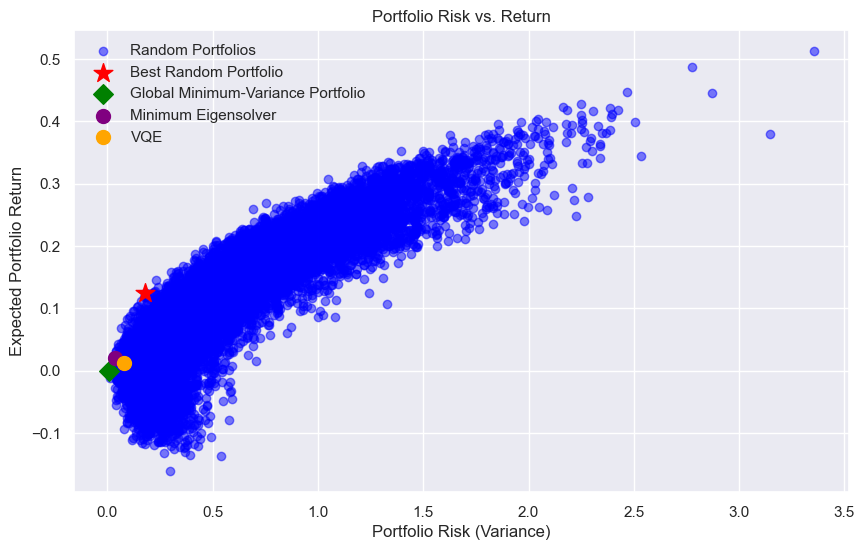
\includegraphics[width=1\columnwidth]{Pictures/allgraphs.png}
\caption{\label{fig:montecarlo} Expected Return of GMVP: -0.0641\%
Risk of GMVP: 0.00889618731780511 Expected Return of Minimum Eigensolver: 2.0669\% Risk of Minimum Eigensolver: 0.03754046707115206 Expected Return of Optimal Portfolio (VQE): 1.2048\% Risk of Optimal Portfolio (VQE): 0.08113489865004302 Expected Return of Monte Carlo: 12.4791\% Risk of Monte Carlo: 0.17700860220543}
\end{figure}


This section presents the performance analysis of four portfolio optimization algorithms: the Global Minimum Variance Portfolio (GMVP), Minimum Eigensolver, Variational Quantum Eigensolver (VQE), and Monte Carlo Simulation. The key performance metrics considered are the expected return and risk (measured as variance) of the optimal portfolios obtained by each method.

\begin{table}[h]
    \centering
    \caption{Performance Metrics of Portfolio Optimization Algorithms}
    \label{tab:performance_metrics}
    \resizebox{\columnwidth}{!}{%
    \begin{tabular}{lcc}
        \hline
        \textbf{Algorithm} & \textbf{Expected Return (\%)} & \textbf{Risk (Variance)} \\
        \hline
        GMVP & -0.0641 & 0.0089 \\
        Minimum Eigensolver & 2.0669 & 0.0375 \\
        VQE (Optimal Portfolio) & 1.2048 & 0.0811 \\
        Monte Carlo Simulation & 12.4791 & 0.1770 \\
        \hline
    \end{tabular}%
    }
\end{table}

The Global Minimum Variance Portfolio (GMVP) algorithm successfully identified the portfolio with the minimum risk, achieving a variance of 0.0089. However, this low level of risk is accompanied by a relatively low expected return of 0.8896\%. This outcome aligns with the GMVP's objective of minimizing risk without explicitly targeting higher returns.

The Minimum Eigensolver approach yielded a portfolio with a higher expected return of 2.0669\% while accepting an increased risk of 0.0375. This method demonstrates a balance between risk and return, allowing for a moderate increase in risk to achieve better returns compared to the GMVP.

The Variational Quantum Eigensolver (VQE) produced an optimal portfolio with an expected return of 1.2048\% and a risk of 0.0811. Although the risk is higher relative to both the GMVP and the Minimum Eigensolver, the expected return is also improved over the GMVP. The VQE results illustrate the potential of quantum algorithms in exploring the trade-off between risk and return in portfolio optimization.

The Monte Carlo Simulation identified a portfolio with the highest expected return of 12.4791\% but also the highest risk of 0.1770. This method explores a wide range of possible portfolio combinations, selecting the best portfolio based on the highest adjusted return. The adjusted return is calculated as:

\begin{equation}
\text{Adjusted Return} = \text{Expected Return} - \lambda \times \text{Risk},
\end{equation}

where the risk factor $\lambda$ is set to 0.5. The high expected return indicates that the Monte Carlo Simulation can find portfolios with superior returns, albeit with increased risk.

These outcomes emphasize the importance of selecting an optimization method that aligns with the investor's risk tolerance and return objectives. Depending on the investment strategy, one may prioritize risk minimization, balanced optimization, or return maximization.

The portfolio risk for each method is calculated using the variance of the portfolio returns:

\begin{equation}
\text{Risk} = \mathbf{w}^\top \Sigma \mathbf{w},
\end{equation}

where $\mathbf{w}$ is the vector of portfolio weights, and $\Sigma$ is the covariance matrix of asset returns. The variance captures the dispersion of portfolio returns and serves as a quantitative measure of risk in this analysis.

In the Monte Carlo Simulation, the adjusted return is employed to identify the best portfolio, balancing the pursuit of high returns with the management of risk. The adjusted return penalizes portfolios with higher risk, as defined by:

\begin{equation}
\text{Adjusted Return} = \mathbf{w}^\top \mathbf{r} - \lambda \times \mathbf{w}^\top \Sigma \mathbf{w},
\end{equation}

where $\mathbf{r}$ is the vector of expected returns, and $\lambda$ is the risk factor (set to 0.5 in this study). By maximizing the adjusted return, the simulation seeks portfolios that offer favorable returns while keeping risk at acceptable levels.

The comparative performance of the algorithms demonstrates varying approaches to portfolio optimization. The GMVP excels in risk minimization but offers lower returns. The Minimum Eigensolver and VQE provide a middle ground between risk and return, allowing for higher expected returns with moderate risk. The Monte Carlo Simulation achieves the highest expected return but with significantly higher risk, highlighting the trade-off between return maximization and risk exposure. Investors can select the appropriate method based on their specific investment goals and risk preferences.




\section{Discussion}
\subsection{Time Complexity}
The GMVP problem is a convex quadratic programming problem, characterized by a quadratic objective function and linear constraints. Solving this problem typically involves the following computational steps:

\begin{enumerate}
    \item \text{Quadratic Programming Solver}: Utilize algorithms such as interior-point methods or active-set methods.
    \item \text{Matrix Operations}: Perform matrix inversions or factorizations, such as Cholesky decomposition of the covariance matrix $\Sigma$.
\end{enumerate}

For dense covariance matrices of size $n \times n$, the dominant computational cost arises from matrix operations, particularly matrix inversion or factorization, which have a time complexity of:

\begin{equation}
T_{\text{GMVP}} = \mathcal{O}(n^3)
\end{equation}

The Minimum Eigensolver method involves finding the minimum eigenvalue and the corresponding eigenvector of the Hamiltonian matrix representing the portfolio optimization problem. The Hamiltonian encapsulates the variance and constraints of the portfolio. Computing the minimum eigenvalue of a dense symmetric matrix (such as the covariance matrix $\Sigma$) requires eigenvalue decomposition algorithms. The computational steps include:

\begin{enumerate}
    \item \text{Eigenvalue Decomposition}: Utilize algorithms like the QR algorithm for dense matrices.
    \item \text{Symmetric Matrix Optimization}: Leverage properties of symmetric matrices to optimize computations.
\end{enumerate}

For dense matrices, the time complexity of eigenvalue decomposition is:

\begin{equation}
T_{\text{Eigensolver}} = \mathcal{O}(n^3)
\end{equation}

The Monte Carlo Simulation method generates $N$ random portfolio allocations and evaluates each to identify the portfolio that maximizes the adjusted return, considering risk. The total time complexity per iteration is dominated by the risk calculation:

\begin{equation}
T_{\text{iteration}} = \mathcal{O}(n^2)
\end{equation}

For $N$ iterations, the total time complexity is:

\begin{equation}
T_{\text{MonteCarlo}} = N \times T_{\text{iteration}} = \mathcal{O}(N n^2)
\end{equation}

The Monte Carlo Simulation method has a time complexity that scales linearly with the number of simulations $N$ and quadratically with the number of assets $n$. By adjusting $N$, one can control the computational effort and the thoroughness of the search.

Next, we will begin by analyzing the time complexity of the SU2 Linear Variational Quantum Eigensolver. In portfolio optimization, each pair of assets contributes to a term in the Hamiltonian due to their covariance, resulting in:
\begin{equation}
K = \frac{n(n+1)}{2} = \mathcal{O}(n^2).
\end{equation}

The Efficient SU(2) ansatz is a hardware-efficient variational form designed to reduce circuit depth and gate complexity, making it suitable for near-term quantum devices. The characteristics of the quantum circuit are as follows:
\begin{itemize}
    \item \text{Circuit Depth} ($D$): Scales linearly with the number of layers $L$:
    \begin{equation}
    D = \mathcal{O}(L).
    \end{equation}
    \item \text{Number of Parameters} ($p$): Scales linearly with the number of qubits $n$ and layers $L$:
    \begin{equation}
    p = \mathcal{O}(nL).
    \end{equation}
    \item \text{Gate Count}: Also scales linearly with $n$ and $L$.
\end{itemize}

Next, we will consider the time complexity involved in  both quantum and classical computational resources. The execution time per quantum circuit is proportional to its depth:
\begin{equation}
T_{\text{circuit}} = \mathcal{O}(D) = \mathcal{O}(L).
\end{equation}
Estimating the expectation value $\langle H \rangle$ requires measuring each term $P_k$ in the Hamiltonian. The total number of measurements $M$ needed to achieve a desired precision $\epsilon$ scales as:
\begin{equation}
M = \mathcal{O}\left( \frac{K}{\epsilon^2} \right).
\end{equation}
This arises from the statistical nature of quantum measurements and the need to estimate expectation values accurately. Combining the measurement requirements with the circuit execution time:
\begin{equation}
T_{\text{measure}} = M \times T_{\text{circuit}} = \mathcal{O}\left( \frac{K}{\epsilon^2} \times L \right).
\end{equation}

The classical optimizer adjusts the parameters $\boldsymbol{\theta}$ to minimize $\langle H \rangle$. The effort depends on:
\begin{itemize}
    \item \text{Number of Parameters} ($p$): $\mathcal{O}(nL)$.
    \item \text{Number of Iterations} ($I$): Depends on the optimizer and problem landscape.
    \item \text{Computational Cost per Iteration}: Generally polynomial in $p$.
\end{itemize}
The classical computation time per iteration, $T_{\text{classical}}$, is usually much less than $T_{\text{measure}}$. The total time per iteration is approximately:
\begin{equation}
T_{\text{iteration}} = T_{\text{measure}} + T_{\text{classical}} \approx T_{\text{measure}}.
\end{equation}
Total time complexity over all iterations:
\begin{equation}
T_{\text{total}} = I \times T_{\text{iteration}} = \mathcal{O}\left( I \times \frac{K}{\epsilon^2} \times L \right).
\end{equation}

For portfolio optimization:
\begin{itemize}
    \item \text{Number of Hamiltonian Terms}: $K = \mathcal{O}(n^2)$.
    \item \text{Circuit Depth}: $L$ is typically constant or increases slowly with $n$.
    \item \text{Total Time Complexity}:
    \begin{equation}
    T_{\text{total}} = \mathcal{O}\left( I \times \frac{n^2}{\epsilon^2} \times L \right).
    \end{equation}
\end{itemize}
Assuming $L$ and $\epsilon$ are constants, the time complexity scales as $\boldsymbol{\mathcal{O}(I n^2)}$

When we compare with traditional classical eigensolvers such as the QR algorithm or the Jacobi method to solve $n \times n$ matrices, we identify that they have a time complexity of $\mathcal{O}(n^3) > \mathcal{O}(I n^2)$. However, the nuance of this statement comes to play for $I$ for different optimization problems. The landscape of portfolio optimization problems play a large factor in how large $I$ is. Given that the time complexity of VQE is $\mathcal{O}(In^2)$, $I$ can be large due to challenges in the optimization landscapes in cases such as barren plateaus, poor ansatz choices, optimizer limitations, and noise or decoherence.

In the presence of barren plateaus, the number of iterations $I$ required for convergence can scale exponentially with the number  of qubits \cite{McClean2018}:

\begin{equation}
    I = \mathcal{O}(\exp(n))
\end{equation}
This will make the time complexity of VQE worse than relevant classical algorithms. To prevent $I$ from being large, using the correct ansatz and avoiding deep circuits are important for implementation of VQE properly on existing quantum hardware. However, there are many methods that can be used to help the performance of $I$ to limit iterations \cite{Grant2019}.

\subsection{Space Complexity}
The space complexity of the GMVP algorithm is determined by the storage requirements of the data structures used in the optimization process:

\begin{enumerate}
    \item \text{Covariance Matrix} $\Sigma$:
    \begin{itemize}
        \item Size: $n \times n$
        \item Space Complexity: $\mathcal{O}(n^2)$
    \end{itemize}
    
    \item \text{Weight Vector} $\mathbf{w}$:
    \begin{itemize}
        \item Size: $n$
        \item Space Complexity: $\mathcal{O}(n)$
    \end{itemize}
    
\end{enumerate}

The dominant factor in the space complexity is the storage of the covariance matrix and related matrices, resulting in a total space complexity of:

\begin{equation}
S_{\text{GMVP}} = \mathcal{O}(n^2)
\end{equation}

The Minimum Eigensolver method involves computing the smallest eigenvalue and the corresponding eigenvector of the Hamiltonian matrix representing the portfolio optimization problem.

Key components affecting space complexity include:

\begin{enumerate}
    \item \text{Hamiltonian Matrix} (or Covariance Matrix) $\Sigma$:
    \begin{itemize}
        \item Size: $n \times n$
        \item Space Complexity: $\mathcal{O}(n^2)$
    \end{itemize}
    
    \item \text{Eigenvectors and Eigenvalues}:
    \begin{itemize}
        \item Storage for eigenvectors (each of size $n$) and eigenvalues (scalars).
        \item For computing all eigenvalues and eigenvectors: Space Complexity $\mathcal{O}(n^2)$
        \item For computing only the smallest eigenvalue and corresponding eigenvector: Space Complexity $\mathcal{O}(n)$
    \end{itemize}
\end{enumerate}

The space complexity is dominated by the need to store the Hamiltonian (covariance) matrix~\cite{Markowitz1952}:

\begin{equation} S_{\text{Eigensolver}} = \mathcal{O}(n^2) \end{equation}

The Monte Carlo Simulation generates $N$ random portfolio allocations, evaluating each to find the portfolio that maximizes the adjusted return~\cite{Boyd2004}.

The space requirements are as follows:

\begin{enumerate} \item \textbf{Covariance Matrix} $\Sigma$: \begin{itemize} \item Size: $n \times n$ \item Space Complexity: $\mathcal{O}(n^2)$ \end{itemize}

\item \textbf{Expected Returns Vector} $\mathbf{r}$:
\begin{itemize}
    \item Size: $n$
    \item Space Complexity: $\mathcal{O}(n)$
\end{itemize}

\item \textbf{Weight Vector} $\mathbf{w}^{(k)}$ for each iteration $k$:
\begin{itemize}
    \item Size per iteration: $n$
    \item Since iterations can be processed sequentially, we need to store only one weight vector at a time.
    \item Space Complexity: $\mathcal{O}(n)$
\end{itemize}
\end{enumerate}

The total space complexity is primarily determined by the storage of the covariance matrix:

\begin{equation} S_{\text{MonteCarlo}} = \mathcal{O}(n^2) \end{equation}

The Variational Quantum Eigensolver (VQE)\cite{Peruzzo2014} is a hybrid quantum-classical algorithm used to find the ground state energy (minimum eigenvalue) of a Hamiltonian. It leverages a parameterized quantum circuit (ansatz) and a classical optimizer\cite{McClean2016}.

The space complexity includes both quantum and classical resources.

\begin{enumerate} \item \textbf{Qubits}: \begin{itemize} \item Number of qubits required depends on the problem encoding. \item For portfolio optimization, each asset may be represented by one or more qubits~\cite{Woerner2019}. \item Assume $n_q$ qubits, where $n_q = \mathcal{O}(n)$. \end{itemize}

\item \textbf{Hamiltonian Representation}:
\begin{itemize}
    \item The Hamiltonian $H$ is expressed as a sum of $K$ Pauli terms:
    \begin{equation}
    H = \sum_{k=1}^{K} h_k P_k
    \end{equation}
    \item Number of terms $K$ depends on the problem; for portfolio optimization, $K = \mathcal{O}(n^2)$~\cite{Hodson2019}.
    \item Storing coefficients $h_k$ and operators $P_k$ requires:
    \begin{itemize}
        \item Coefficients: $\mathcal{O}(K)$
        \item Operators: Each $P_k$ acts on $n_q$ qubits; storing requires $\mathcal{O}(n_q K)$ bits if using binary representation.
    \end{itemize}
    \item Total Space Complexity for Hamiltonian: $\mathcal{O}(n^2)$
\end{itemize}

\item \textbf{Variational Parameters} $\boldsymbol{\theta}$:
\begin{itemize}
    \item Number of parameters depends on the ansatz.
    \item For the Efficient SU(2) ansatz, the number of parameters scales as:
    \begin{equation}
    p = \mathcal{O}(n_q L)
    \end{equation}
    where $L$ is the number of layers (typically constant or slowly increasing with $n$)~\cite{Kandala2017}.
    \item Space Complexity: $\mathcal{O}(n)$
\end{itemize}

\item \textbf{Classical Optimization Data}:
\begin{itemize}
    \item Storage for gradients, intermediate variables in the optimizer.
    \item Space Complexity: $\mathcal{O}(n)$
\end{itemize}
\end{enumerate}

\begin{equation} S_{\text{VQE}}^{\text{Quantum}} = \mathcal{O}(n) \end{equation}

\begin{equation} S_{\text{VQE}}^{\text{Classical}} = \mathcal{O}(n^2) \end{equation}

The overall space complexity is dominated by the storage of the Hamiltonian on the classical computer.

\section{Conclusion}

Current Noisy Intermediate-Scale Quantum (NISQ) devices~\cite{Preskill2018} are not yet capable of efficiently handling large-scale portfolio optimization problems involving more than ten assets, especially when selecting a subset from the larger set. Nevertheless, theoretical developments suggest that quantum algorithms can achieve quadratic speedups in both time and space complexities for such optimization tasks~\cite{Harrow2009}. For instance, utilizing a linear SU(2) ansatz with a circuit depth of 32 demonstrates favorable properties, as the circuit depth scales linearly with the number of qubits, which is advantageous for scalability~\cite{Kandala2017}.

Exploring alternative quantum computing platforms, such as quantum annealing and Grover Adaptive Search (GAS), may offer additional benefits over current methods~\cite{Farhi2000,Grover1996}. While algorithms like the Quantum Approximate Optimization Algorithm (QAOA) are valuable~\cite{Farhi2014}, they may not provide significant advantages in this context due to their specific focus. The rich landscape of SU($n$) ansatz presents ample opportunities for further research, as different ansatz can be optimized to solve various Hamiltonians more effectively, tailoring the quantum algorithm to the problem's specific requirements~\cite{Cerezo2021}.

From a scalability perspective, quantum algorithms exhibit promising characteristics with potential quadratic speedups in time, making them suitable candidates for large-scale optimization problems~\cite{Shor1997}. However, the performance of these algorithms is highly dependent on the underlying quantum hardware~\cite{Devitt2016}. Transpilation studies reveal that the choice of quantum processor significantly influences the accuracy and efficiency of the implemented ansatz~\cite{Tannu2019}. For example, on IBM's Brisbane superconducting quantum processor~\cite{IBMQBrisbane}, certain quantum circuits perform better or worse due to the specific connectivity and properties of the superconducting qubits~\cite{Krinner2019}.

In summary, while current quantum hardware imposes limitations, the theoretical foundations and potential scalability of quantum algorithms for portfolio optimization are encouraging~\cite{Woerner2019}. Future advancements in quantum hardware and algorithm design, particularly through the exploration of diverse ansatz and hardware-specific optimizations, are expected to overcome existing challenges and unlock the full potential of quantum computing in this domain~\cite{Bharti2022}.

\appendix \section*{Code Availability}

All code used in this study, including the implementations of the Variational Quantum Eigensolver (VQE) and other quantum algorithms for portfolio optimization, is available on GitHub. Interested readers and researchers are encouraged to explore the repository to verify results, replicate experiments, or modify the code for further experimentation.

You can access the repository at the following link: \begin{center} \url{https://github.com/Lion-Q/finance-qbraid} \end{center}

We welcome contributions and suggestions for improving the code. Please feel free to open issues or submit pull requests if you encounter any bugs or have ideas for enhancements.



\bibliographystyle{unsrt} \bibliography{references}

\end{document}